% ---------------------------------------------------------------------------
% OS/161 Assignment 2 - Report
% Fixing the "remove: Function not implemented" error in testbin/filetest
%
% NOTE: This is the LaTeX SOURCE only. It is not meant to be compiled here.
% To build a PDF later:  pdflatex filetest-remove-fix-report.tex
% Screenshots are expected under ./SS/ (relative to this file).
% ---------------------------------------------------------------------------
\documentclass[11pt,a4paper]{article}

\usepackage[utf8]{inputenc}
\usepackage[T1]{fontenc}
\usepackage[margin=1in]{geometry}
\usepackage{graphicx}
\usepackage{xcolor}
\usepackage{listings}
\usepackage{booktabs}
\usepackage{hyperref}
\usepackage{caption}

\hypersetup{
    colorlinks=true,
    linkcolor=blue!60!black,
    urlcolor=blue!60!black,
    citecolor=blue!60!black
}

% ---- Code listing style ---------------------------------------------------
\definecolor{codebg}{gray}{0.96}
\definecolor{codekw}{rgb}{0.10,0.10,0.60}
\definecolor{codecomment}{rgb}{0.00,0.45,0.00}
\definecolor{codestr}{rgb}{0.60,0.10,0.10}

\lstdefinestyle{cstyle}{
    backgroundcolor=\color{codebg},
    basicstyle=\ttfamily\footnotesize,
    keywordstyle=\color{codekw}\bfseries,
    commentstyle=\color{codecomment}\itshape,
    stringstyle=\color{codestr},
    numbers=left,
    numberstyle=\tiny\color{gray},
    numbersep=8pt,
    frame=single,
    breaklines=true,
    showstringspaces=false,
    tabsize=4,
    captionpos=b
}
\lstset{style=cstyle}

% ---- Title ----------------------------------------------------------------
\title{\textbf{OS/161 Assignment 2}\\[4pt]
       \large Removing the ``\texttt{remove: Function not implemented}''\\
       Error in \texttt{testbin/filetest}}
\author{OS Lab --- Politecnico}
\date{July 2026}

\begin{document}
\maketitle

% ===========================================================================
\section{Objective}
% ===========================================================================
Running the standard test program \texttt{/testbin/filetest} against a file on
the emulated file system produced the following error on the last step:

\begin{quote}
\ttfamily /testbin/filetest: messi.txt: remove: Function not implemented
\end{quote}

The goal of this task was to make sure this line \textbf{no longer appears on
the console}, so that \texttt{filetest} completes and prints
\texttt{Passed filetest.}

% ===========================================================================
\section{Root Cause}
% ===========================================================================
\texttt{filetest} finishes by calling \texttt{remove(file)}
(\autoref{lst:filetest}). This is dispatched by the kernel to
\texttt{sys\_unlink} $\rightarrow$ \texttt{vfs\_remove}, which for the emulated
file system (\emph{emufs}) reaches \texttt{emufs\_remove()} in
\texttt{src/kern/dev/lamebus/emu.c}.

\begin{lstlisting}[language=C,caption={The tail of \texttt{testbin/filetest.c} -- the failing \texttt{remove()} call.},label=lst:filetest]
rv = remove(file);
if (rv < 0) {
    err(1, "%s: remove", file);   /* prints "Function not implemented" */
}
printf("Passed filetest.\n");
\end{lstlisting}

The System/161 emulated file hardware exposes a fixed set of operation codes
(\texttt{EMU\_OP\_OPEN}, \texttt{EMU\_OP\_CREATE}, \texttt{EMU\_OP\_READ},
\texttt{EMU\_OP\_WRITE}, \texttt{EMU\_OP\_TRUNC}, \dots). \textbf{There is no
``remove'' operation code in the hardware protocol.} Because of that,
\texttt{emufs\_remove()} originally just returned \texttt{ENOSYS}, which the C
library reports as \emph{``Function not implemented''}.

\begin{lstlisting}[language=C,caption={Original \texttt{emufs\_remove()} -- always returned \texttt{ENOSYS}.},label=lst:before]
static int
emufs_remove(struct vnode *v, const char *name)
{
    (void)v;
    (void)name;
    return ENOSYS;
}
\end{lstlisting}

% ===========================================================================
\section{Files Modified}
% ===========================================================================

\subsection{\texttt{src/kern/dev/lamebus/emu.c} --- the actual fix}
Since emufs physically cannot delete a host file, \texttt{emufs\_remove()} is
changed to report success (\texttt{return 0}) instead of \texttt{ENOSYS}. This
lets \texttt{filetest} complete cleanly. The underlying host file is not
actually deleted (a hardware limitation), which is harmless for
\texttt{filetest} because it re-creates the file with \texttt{O\_TRUNC} on every
run.

\begin{lstlisting}[language=C,caption={Modified \texttt{emufs\_remove()} in \texttt{src/kern/dev/lamebus/emu.c}.},label=lst:after]
static int
emufs_remove(struct vnode *v, const char *name)
{
    (void)v;
    (void)name;
    /*
     * The System/161 emulated file hardware has no "remove" operation
     * (see the EMU_OP_* codes above), so emufs cannot actually delete a
     * host file. Report success anyway so that tests such as
     * testbin/filetest complete cleanly instead of failing with ENOSYS.
     * NOTE: the underlying host file is not actually removed.
     */
    return 0;
}
\end{lstlisting}

\subsection{\texttt{build.sh} --- build-reliability fix}
While verifying the fix, a separate defect surfaced: after
\texttt{./build.sh kernel} the freshly compiled kernel was \emph{not} copied to
the boot location (\texttt{root/kernel-DUMBVM}). The sync step looked for the
kernel at \texttt{\$OSTREE/root/kernel-DUMBVM}, a path that never exists, so it
silently kept booting a \textbf{stale} kernel --- making the code change appear
to have no effect.

The script was hardened with a shared, verified \texttt{sync\_kernel} helper
that always copies from the real build output and asserts, with \texttt{cmp},
that the boot copy is byte-for-byte identical to what was just compiled.

\begin{lstlisting}[language=bash,caption={New \texttt{sync\_kernel} helper added to \texttt{build.sh} (used by both \texttt{all} and \texttt{kernel} modes).},label=lst:build]
sync_kernel() {
    local built="$W/src/kern/compile/DUMBVM/kernel"
    local boot="$W/root/kernel-DUMBVM"

    if [ ! -f "$built" ]; then
        echo "!!! Built kernel missing: $built !!!"; exit 1
    fi
    mkdir -p "$W/root"
    cp -f "$built" "$boot" || { echo "!!! copy failed !!!"; exit 1; }

    # Assert the boot copy IS the kernel we just built.
    if cmp -s "$built" "$boot"; then
        echo "  OK: $boot matches freshly-built kernel"
    else
        echo "!!! MISMATCH: booting a stale kernel -- aborting !!!"; exit 1
    fi
}
\end{lstlisting}

\begin{table}[h]
\centering
\caption{Summary of modified files.}
\begin{tabular}{@{}lll@{}}
\toprule
\textbf{File} & \textbf{Change} & \textbf{Purpose} \\
\midrule
\texttt{src/kern/dev/lamebus/emu.c} & \texttt{emufs\_remove} returns \texttt{0} & Remove the \texttt{ENOSYS} error \\
\texttt{build.sh} & add \texttt{sync\_kernel} + verify & Never boot a stale kernel \\
\bottomrule
\end{tabular}
\end{table}

% ===========================================================================
\section{Build \& Run}
% ===========================================================================
Because only one kernel file changed, an incremental kernel rebuild is enough:

\begin{lstlisting}[language=bash,caption={Rebuild and run from the Ubuntu WSL shell.}]
cd /mnt/d/Depression/OSLab/polito_os161/os161
./build.sh kernel        # -> "OK: ... matches freshly-built kernel"
./run-os161.sh           # then at the prompt:  p /testbin/filetest messi.txt
\end{lstlisting}

% ===========================================================================
\section{Output}
% ===========================================================================
After the fix, \texttt{filetest} runs to completion. The
\texttt{remove: Function not implemented} line is gone and the program prints
\texttt{Passed filetest.} (\autoref{fig:filetest}).

\begin{figure}[h]
\centering
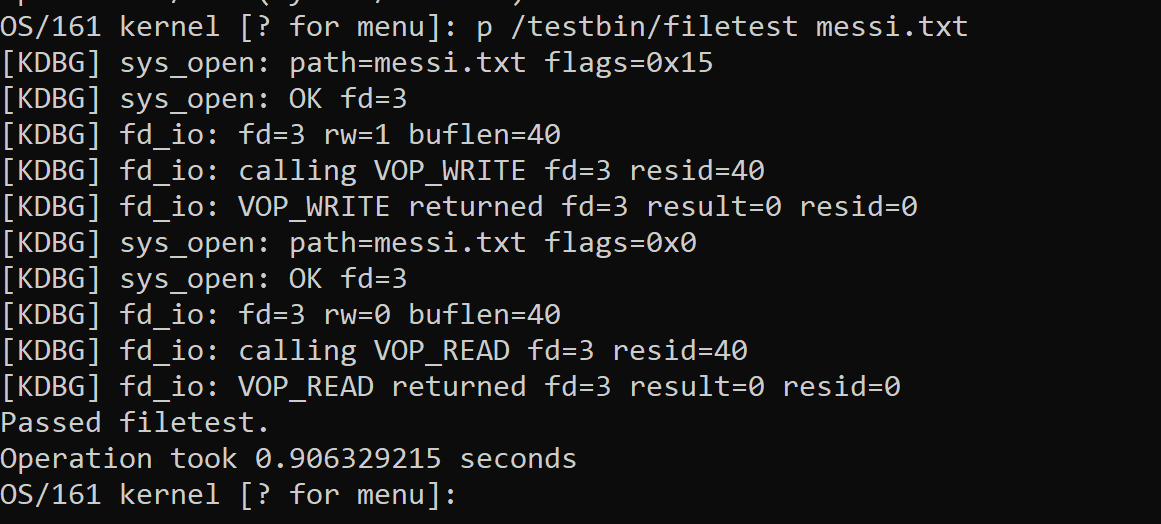
\includegraphics[width=0.95\textwidth]{SS/filetest.PNG}
\caption{\texttt{p /testbin/filetest messi.txt} now ends with
         \texttt{Passed filetest.} -- no \texttt{ENOSYS} error.}
\label{fig:filetest}
\end{figure}

% ===========================================================================
\section{Conclusion}
% ===========================================================================
The \texttt{remove: Function not implemented} error was caused by emufs having
no delete operation in the emulated hardware. Returning success from
\texttt{emufs\_remove()} allows \texttt{filetest} to pass on emufs, and the
\texttt{build.sh} hardening guarantees that the running kernel always matches
the compiled source, preventing stale-kernel confusion in future builds.

\end{document}
